%% paper/sections/method.tex
%% Draft only. Architecture description; no results numbers here.
\label{sec:method}

\subsection{Entity-Persistent Tokenization}
Entity-Persistent Tokenization (EPT) replaces a video's spatial patch grid
with a small set of tokens indexed by \emph{(entity, segment)} rather than
\emph{(spatial cell, frame)}. A detector and tracker (or, for datasets with
shot cuts, a detector plus identity clustering) locate up to $E$ entities per
clip and assign each detected instance to one of $S$ temporal segments. Entity
selection is fixed and identical across every condition that uses it: the top
$E$ tracks by confidence $\times$ frame-coverage, so the same $E$ tracks are
selected regardless of what happens to them downstream. Each cached token is
the frozen backbone's CLS token concatenated with its mean-pooled patch
tokens, averaged over all detections of that entity within that segment; a
token whose entity is absent from a given segment is marked in a companion
presence mask rather than zero-filled and silently attended over. Every
condition in this paper, including the spatial-grid baseline (A0), consumes
identical cached backbone features — the same encoder, the same crop
preprocessing, the same feature cache — so any measured difference is
attributable to tokenization structure, not to encoder capacity
(\S\ref{sec:pre-registration}).

\subsection{The EPT-Former}
\begin{figure}[t]
  \centering
  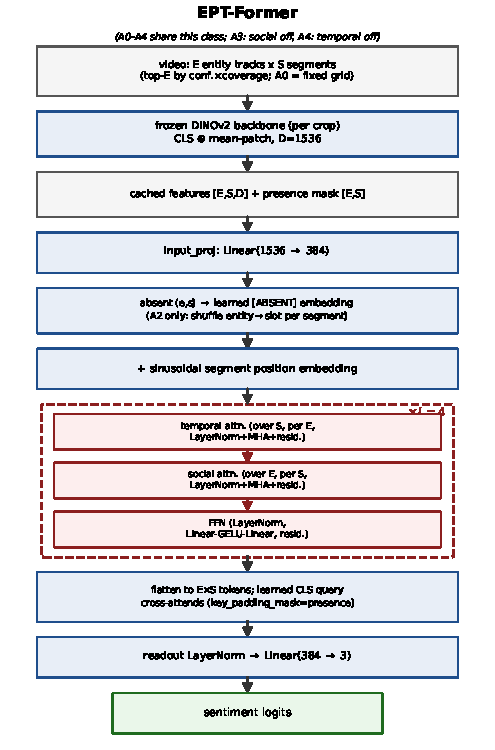
\includegraphics[width=\linewidth]{figures/fig1_architecture.pdf}
  \caption{EPT-Former forward pass. A0 and A1--A4 share this class, differing
    only in \texttt{use\_temporal}/\texttt{use\_social} and, for A0 vs.\
    A1/A3/A4, the token source (grid vs.\ entity crops).}
  \label{fig:architecture}
\end{figure}
The EPT-Former consumes the cached $[E, S, D]$ feature tensor and its
presence mask. Features are linearly projected to $d{=}384$; absent
$(e,s)$ positions are replaced with a single learned \texttt{[ABSENT]}
vector, shared across all entities and segments, before a sinusoidal
segment-position embedding is added. $L{=}4$ blocks follow, each performing
multi-head attention~\cite{vaswani2017attention} temporally (over $S$,
independently per entity), then socially (over $E$, independently per
segment), then a feed-forward layer --- 6 heads, MLP ratio 4, pre-norm
throughout. A learned CLS query
cross-attends over the flattened $E{\times}S$ token set (masked by presence)
for readout, followed by a linear classifier. Figure~\ref{fig:architecture}
diagrams the full forward pass. The whole head is
%% results/efficiency.csv: attention_stack_params column, A1 row (10652163)
10.65M parameters, independent of $E$ and $S$ (the block weights are shared
across entity and segment positions).

Two structural choices are load-bearing for the control in
\S\ref{sec:shuffle-control} and are enforced by a construction-time check,
not just a convention: \textbf{no learned per-slot identity embedding}
exists anywhere in the model (a parameter indexed by entity-slot position
would let the network recover identity from slot position alone, independent
of the token content, confounding the persistence test), and slot order is
never treated as informative --- the model is architecturally identical
whether entity $e$ occupies slot 0 or slot 5 in any given sample.

\subsection{Isolating Persistence: the Identity-Shuffle Control}
\label{sec:shuffle-control}
The question this paper asks is not ``do entity-localized tokens help'' but
specifically ``does \emph{persistent identity} across segments help, as
opposed to entity-localized cropping and a smaller token budget, which
travel with it by default.'' A1 and A0 alone cannot separate these: A0 uses
a fixed spatial grid (no entities, no persistence, a different --- typically
larger --- token count), so any A1--A0 gap is consistent with either
explanation and cannot distinguish them.

A2 isolates persistence directly: it is architecturally identical to A1 ---
same backbone features, same token count, same entity-localized crops, same
EPT-Former weights and hyperparameters --- with exactly one difference. The
entity-to-slot assignment is shuffled independently per segment, using a
deterministic per-clip seed derived from the run seed
(\texttt{shuffle\_entities\_per\_segment}, applied identically to the
feature tensor and its presence mask). The entity occupying slot 3 in
segment 1 is, in general, a different physical entity than the one occupying
slot 3 in segment 2 --- the model still receives entity-localized,
matched-budget tokens, it just can no longer track any one entity's state
across segments, because ``the token in this slot'' no longer refers to the
same tracked identity from one segment to the next. Any gap between A1 and
A2 is therefore attributable to persistence and only to persistence
(H1, \S\ref{sec:pre-registration}); any gap between A1/A2 and A0 is
attributable to entity localization and token budget, independent of
whether persistence itself does anything (H2).
